%\clearpage
%\section{Обзор литературы}
%
%\subsection{Механизмы усложнения организации генома}
%
%Помимо стандартного варианта созревания РНК путем сохранения экзонов и сплайсосомного вырезания интронов из первичного транскрипта, существуют варианты, отличающиеся от канонического.
%Одним из таких вариантов является альтернативный сплайсинг - основной источник транскрипционной изменчивости, когда одному гену может соответствовать несколько транскриптов.
%Кроме общеизвестного ``удержания интрона`` (intron retention (IR)), важно обозначить такой процесс, как альтернативное полиаденилирование, так как оно также оказывает прямое влияние на вариативность транскриптов~\cite{Mamon2019}.
%
%Альтернативный сплайсинг (alternative splicing (AS)) достаточно распространен у эукариот.
%Данный механизм способствует увеличению белкового разнообразия у организма.
%Выделяют следующие типы альтернативного сплайсинга: т.н. ``пропуск экзонов``; вариант, когда используются наборы из нескольких экзонов, расположенных рядом друг с другом и  формирующих кассеты, при этом во время сплайсинга выбирается только один из нескольких экзонов в каждой из кассет; также могут использоваться различные 5'- и 3'-сайты сплайсинга в интронах или экзонах, выбор которых зависит от цис- и транс-действующих факторов, необходимых для формирования сплайсосомы~\cite{Mamon2019}.
%
%``Удержание интрона`` является одним из вариантов альтернативного сплайсинга, который распространен у млекопитающих.
%Данный механизм увеличивает сложность транскриптома~\cite{Schmitz2017}, но часто в интронах присутствуют кодоны преждевременной терминации (premature termination codons (PTCs)) внутри основной открытой рамки считывания.
%В результате возможно 2 исхода: нонсенс-опосредованный распад мРНК с сохраненным интроном или продукция укороченных белков~\cite{Mamon2019}.
%Именно эти варианты интересуют нас больше всего.
%Такие мРНК с оставшимся интроном дают альтернативные формы белков, а значит являются источником функционального разнообразия генных продуктов, что демонстрирует важность интронов как структурной единицы гена.
%Для разных организмов показано, что наличие такой мРНК с интроном для гена \textit{Nxf1} является консервативным признаком~\cite{Mamon2013}, о чем речь пойдет далее.
%
%
%\subsection{Значимость интронов}
%
%Интроны делят на 3 группы: I, II, III.
%Интроны I и II группы обнаруживаются в геномах некоторых бактерий и органелл.
%Интроны I группы также обнаружены в рибосомных РНК (рРНК) ядер протистов и грибов.
%Эти две группы имеют разные структуры РНК, которые облегчают их активность самосплайсинга.
%Они также содержат внутренние открытые рамки считывания (open reading frame (ORF)), которые облегчают как удаление интронов из транскриптов РНК, так и распространение интронов на безинтронные сайты посредством обратной транскрипции~\cite{Roy2006}.
%Третья же группа интронов – сплайсосомные интроны – найдены в ядерных геномах всех охарактеризованных эукариот.
%Обычно они не имеют открытых рамок считывания и их удаление происходит с помощью сплайсосомы~\cite{Jurica2013}.
%
%К непосредственным функциям интронов можно отнести следующее.
%Во-первых, это положительная регуляция экспрессии генов.
%Впервые данное явление было продемонстрировано очень давно в эксперименте с использованием конструкций вируса SV40, где показали, что количество белка было значительно снижено без его интронов~\cite{Gruss1979}.
%В последующем это было также показано на дрожжах и млекопитающих~\cite{Juneau2006}.
%
%Во-вторых, можно отнести регуляцию нонсенс-опосредованного распада мРНК, который был упомянут при описании удержания интрона.
%Обычно NMD описывают, как механизм надзора у эукариот, который избирательно удаляет мРНК, содержащие ошибочно сгенерированные PTCs~\cite{Jo2015}.
%Однако, есть доказательства в пользу того, что интроны, расположенные в 5'- или 3'-нетранслируемых областях (untranslated region (UTR)), играют важную роль в контроле NMD-чувствительности транскриптов~\cite{Kalyna2012}.
%
%В-третьих, интроны могут быть связаны с транспортом мРНК.
%Раньше считалось, что сплайсированные транскрипты быстрее экспортируются из ядра в цитоплазму, однако были и противоречивые исследования~\cite{Jo2015}.
%Один из относительно недавних экспериментов с использованием флуоресцентной гибридизацией in situ (FISH) показал, что несущие интроны транскрипты преимущественно расположены в цитоплазме~\cite{Valencia2008}, что сильнее подвергает сомнению высказанные ранее гипотезы и требует их пересмотра.
%
%Помимо перечисленных функций есть также предположение о том, что часть последовательностей концов интронов может быть ответственна за истощение нуклеосом в интронах путем отталкивания нуклеосом в сторону экзонов~\cite{Schwartz2009}.
%Это позволяет задуматься о роли интронов в сборке хроматина.
%
%Стоит отметить порядковое положение интронов в гене.
%Больше всего внимание привлекает первый интрон среди всех интронов гена, обычно именно он обладает особыми функциональными характеристиками~\cite{Jo2015}.
%Например, первый интрон гена \textit{oskar} Drosophila играет важную роль в правильной цитоплазматической локализации некоторых мРНК~\cite{Siemens2004}.
%
%Длина интронов также является важной характеристикой.
%Есть предположение о том, что длинные интроны повышают эффективность естественного отбора, устраняя интерференцию Хилла-Робертсона~\cite{Comeron2008}.
%
%В одной из работ десятилетней давности на дрожжах \textit{Saccharomyces cerevisiae} наблюдали, как короткие ORF могут эволюционировать в настоящие функциональные гены посредством своего рода непрерывного эволюционного процесса~\cite{Carvunis2012}.
%Это позволило предположить, что интроны могут стать источником новых генов.
%
%В наше время активно используется метод полногеномного поиска ассоциаций, сокращенно GWAS – genome-wide association study.
%В основе метода лежит сравнительный анализ однонуклеотидных вариантов (single-nucleotide variant (SNV)), а точнее участков в геноме, которые схожи между собой по этим однонуклеотидным заменам, между индивидуумами~\cite{Smith2019}.
%Примечательно, что при картировании аллелей, ассоциированных с какими-то заболеваниями, место картирования соответствует именно интронным областям~\cite{Welter2014}.
%Данный факт является очередным подтверждением важности изучения интронов.
%
%
%\subsection{Семейство генов \textit{Nxf}, общая характеристика}
%
%Принимая во внимание все выше сказанное, можно перейти к описанию основного объекта, на который направлено данное исследование.
%Перед этим стоит сказать несколько вводных слов про само семейство.
%
%Семейство генов \textit{Nxf} (nuclear export factor) было названо в честь функции универсального гена \textit{Nxf1}, продукт которого ответственен за ядерно-цитоплазматический транспорт большинства мРНК.
%Гены данного семейства обнаружены у всех эукариотических организмов группы Opisthokonta и характеризуются эволюционной консервативностью~\cite{Mamon2013}.
%
%Геномы различных грибов имеют лишь один ген-представитель этого семейства, растения и некоторые простейшие вовсе их лишены.
%Животные, как правило, имеют от двух до пяти паралогичных генов~\cite{Mamon2013}.
%
%Характерной особенностью для гена Nxf1 является существование транскриптов с невырезанным гомологичным интроном.
%Особое внимание выделяется консервативному блоку, состоящему из последовательно идущих экзонов размером 110 п.н. и 37 п.н., а также интрону, который находится между ними и который принято называть ``кассетным``~\cite{Mamon2013}.
%Соответственно, сам блок из трех единиц мы будем называть ``консервативной кассетой``.
%
%Среди животных, для которых есть данные про семейство генов Nxf, были выявлены 3 таксономические группы, и в каждой из них кассетный интрон имеет определенные характеристики~\cite{Mamon2013}.
%
%К первой группе относятся позвоночные, для них характерен интрон, находящийся между 10-м и 11-м экзонами в гене \textit{Nxf1}.
%В интроне позвоночных выявили 4 участка протяженной гомологии: 1) 5´-концевая последовательность; 2) фрагмент, содержащий конститутивный транспортный элемент (constitutive transport element (СТЕ), характерный для ретровирусов; 3) третий консервативный участок; 4) 3´-концевая последовательность~\cite{Mamon2013}.
%
%Ко второй группе принадлежат дрозофилиды с кассетным интроном 5-м в генах \textit{Nxf1}.
%Несмотря на отсутствие участков протяженной гомологии, что характерно для позвоночных, у разных видов Drosophilidae есть схожая черта – две протяженные последовательности, обогащенные аденином (А).
%Предполагается, что вторичная структура транскриптов с сохраненным интроном, образовавшаяся за счет наличия этих последовательностей, способствует их сохранению~\cite{Mamon2013}.
%
%В последнюю группу включены нематоды с интроном 5-м или 6-м.
%Его размер на порядок меньше, а участки протяженной гомологии не обнаружены.
%Однако, внутри группы есть общее сходство – это повышенное содержание тимина (Т), что отличает данную группу организмов от остальных~\cite{Mamon2013}.
%
%Как уже упоминалось ранее, важной особенностью для генов Nxf1 у позвоночных и дрозофилид является способность к образованию сложных вторичных структур, которая может играть существенную роль в пост-транскрипционной судьбе транскрипта~\cite{Golubkova2012}.
%Помимо этого, все же главной особенностью, кроме сохраненного интрона в транскрипте, становится наличие в этом сохранившемся интроне преждевременного стоп-кодона, но мРНК избегает нонсенс-опосредованного распада, и в итоге возможно образование укороченного белка.
%Перейдем к подробному рассмотрению гена \textit{Nxf1}.
%
%
%\subsection{Структура и функции Nxf1 (гена и белка)}
%
%Первоначально белок Nxf1 у людей был идентифицирован как потенциальный цитоплазматический кофактор для Tip (белок, взаимодействующий с тирозинкиназой), кодируемый вирусом герпеса saimiri, и был назван TAP (Tip-associated protein, или белок, ассоциированный с Tip)~\cite{Yoon1997}.
%Позже было показано, что ТАР участвует в ядерно- цитоплазматическом транспорте несплайсированной или частично сплайсированной РНК ретровирусов.
%TAP напрямую распознает только одну последовательность – CTE, которая была первоначально обнаружена в РНК ретровирусов~\cite{Zolotukhin2001}.
%Мы предполагаем, что функцию CTE у дрозофилид выполняет образуемая благодаря сохранению интрона вторичная структура.
%На данный момент наилучшее представление о гене \textit{Nxf1} есть для дрозофилид и млекопитающих.
%Рассмотрим функцию и организацию данного гена, а также белковые домены для \textit{Drosophila melanogaster} и \textit{Homo sapiens}.
%
%Nxf1 имеет модульную доменную организацию (на Рис.~\ref{fig:dm_hs_nxf1_structure} представлена структура гена, последовательности в котором кодируют белковую структуру), состоящую из РНК-связывающего домена (RBD), четырех богатых лейцином повторов (LRR), домена, проявляющего сходство с ядерным транспортным фактором 2 (NTF2-подобный домен), и С-концевой убиквитин-ассоциированный, или UBA-подобный, домен~\cite{Mamon2013}.
%
%\begin{figure}[h] % here, top, bottom, page
%    \centering
%    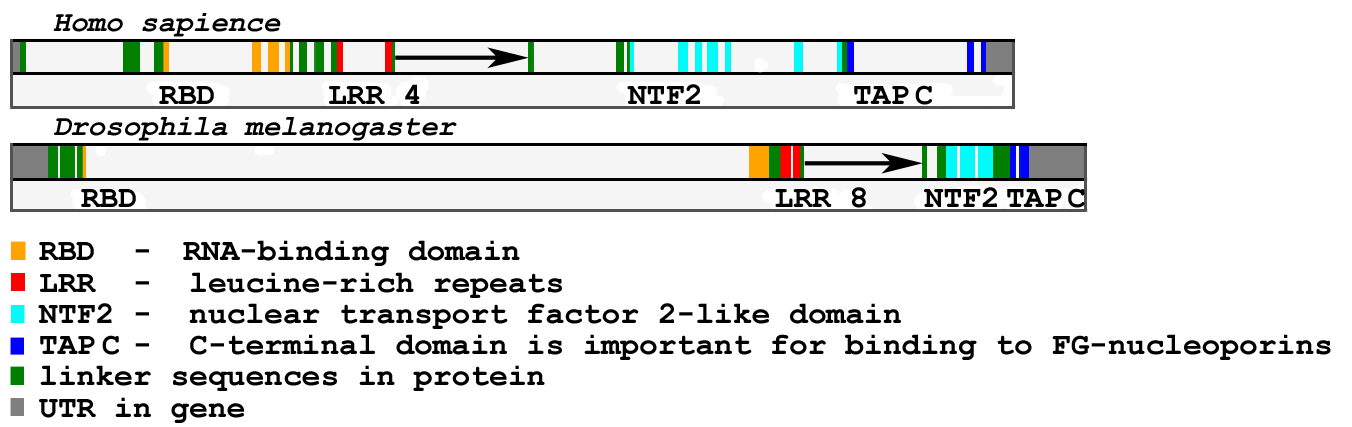
\includegraphics[width=0.9\textwidth]{images/dm_hs_nxf1_structure}
%    \caption{Интрон-экзонная структура для генов \textit{Hs Nxf1} и \textit{Dm Nxf1}. Стрелки обозначают ``кассетный`` интрон. Цвета экзонов отображают белковые домены~\cite{Mamon2013}.}
%    \label{fig:dm_hs_nxf1_structure}
%\end{figure}
%
%Основной и общеизвестной функцией продукта гена \textit{Nxf1} является транспорт всех типов мРНК из ядра в цитоплазму~\cite{Herold2000}.
%Кассетный интрон условно разделяет \textit{Nxf1} на две функциональные половины – рецепторную, куда относятся RBD и LRR, отвечающую за взаимодействие с РНК, и транспортную, куда входят NTF2L и UBA, позволяющую, взаимодействуя с другими белками, обеспечивать транспорт комплекса макромолекул через ядерные поры~\cite{Mamon2013}.
%
%Помимо классической функции нашей группой выявлены дополнительные, жизненно важные функции продукта гена \textit{Nxf1}, или \textit{sbr} у дрозофилид.
%Во-первых, доказано, что sbr выполняет семенниково-специфические функции.
%Показано, что существуют специфичные для семенников альтернативные транскрипты, полученные за счет альтернативного промотора, этого гена и укороченный белок sbr, обнаруженный только в семенниках~\cite{Ginanova2016}.
%
%Во-вторых, установлено, что белок sbr необходим для формирования внутренней структуры и установления границ в мозговом веществе зрительной системы дрозофилы.
%Распределение sbr в ядре и цитоплазме специфических нейронов и глиальных клеток свидетельствует о специализированных функциях этого белка~\cite{Mamon2021}.
%
%Также в одной из недавних работ была продемонстрирована значимость ``кассетного`` интрона в эволюции гена \textit{Nxf1} у представителей Chiroptera~\cite{Bondaruk2022}.
%
%В моей бакалаврской работе было проанализировано 89 нуклеотидных последовательностей гена \textit{Nxf1} из таксономической группы Arthropoda, а также найдены последовательности гена для 37 представителей дрозофилид.
%По результатам проведенных множественных выравниваний и построенных вторичных структур интрон-содержащего транскрипта были сформулированы следующие выводы:
%
%\begin{enumerate}[left=\parindent]
%    \item Структура ``консервативной кассеты`` является специфической для таксонов низкого ранга у всех взятых в анализ артропод.
%    \item Интрон-содержащие транскрипты формируют специфические вторичные структуры; у дрозофилид продемонстрировано наличие А-обогащенных участков.
%\end{enumerate}
%
%Таким образом, важность роли гена \textit{Nxf1} и ``кассетного`` интрона в нем не вызывает сомнений.
%Тем не менее очень интересно было бы проанализировать структуру данного гена у представителей за пределами Arthropoda, используя современные методы биоинформатики, освоенные в магистратуре, о чем и пойдет речь далее.
